\section{Membuat Kembalian Web Service Dalam Bentuk JSON Pada HTTP GET,  POST, PUT, dan DELETE}
\subsection{Definisi JSON}
JavaScript Object Nation atau biasa dikenal dengan JSON ialah sebuah format untuk berbagi data. Sesuai namanya, JSON merupakan turunan dari JavaScript, tetapi format ini tersedia untuk beberapa bahasa pemrograman lain, di antaranya: Python, PHP, Ruby, dan Java. JSON biasanya dilafalkan menjadi ‘Jason’. JSON memiliki format file .json saat ia bersiri sendiri. Akan tetapi jika didefinisikan ke dalam format lain semisal .html, ia dapat ditampilkan dalam tanda petik sebagai JSON string, atau JSON ini juga bisa dimasukkan ke dalam sebuah variabel. Format ini sangat mudah untuk ditransfer antar server web dengan klien atau browser. 

Karena sangat ringan dan mudah dibaca, JSON bisa memberikan alternatif lebih baik dari XML dan tidak membutuhkan formatting yang tidak banyak. Panduan ini dapat membantu pembaca untuk memahami apa itu JSON, bagaimana menggunakan data di file JSON, dan struktur serta sintaks dari format ini. JSON juga merupakan format yang ringan dan mempermudah segala sesuatu supaya dapat membagi, menyimpan dan bekerja dengan data. Sebagi sebuah format, JSON telah mendapatkan dukungan yang makin meningkat dalam bentuk API, misalnya di Twitter API.

Karena mungkin akan jarang membuat file .json sendiri namun mengunduhnya dari sumber lain, pikirkan bagaimana menggunakan JSON dengan baik diprogram daripada memikirkan strukturnya.

\subsection{Sintaks dan Struktur} 
Objek dari JSON adalah format data key-value yang biasanya dirender di dalam kurung kurawal. Saat mengerjakan file JSON, mungkin akan sering melihat objek JSON disimpan sebagai objek JSON atau string di dalam sebuah program.
Contoh objek JSON seperti pada listing \ref{lst:ojson}:
\lstinputlisting[caption=Contoh Objek JSON,label={lst:ojson}]{src/12/ojson.py}

Walaupun contoh di atas merupakan contoh singkat dan JSON dapat memiliki isi yang sangat banyak. Secara umum, contoh di atas menggambarkan dua kurung kurawal (\{\}) di awal dan akhir dengan pasangan key-value di antara kedua tanda kurang. Sebagian data yang dipakai di JSON dienkapsulasi di dalam sebuah objek JSON.

Yang di sebut Key JSON yaitu berada di sebelah kiri titik dua. Mereka perlu dilengkapi oleh tanda petik dua seperti ini: “key”. Key dapat berupa string apa pun dengan syarat string valid. Dalam sebuah objek, key harus bersifat unik. Key juga bisa berupa spasi seperti “first name”, namun disarankan jangan menambahkan spasi karena ini akan membuat repot saat menjalankan kode, lebih baik menggunakan underscore seperti ini: “first\_name”.
\begin{enumerate}
\item Value JSON terletak di sebelah kanan setelah titik dua. Ada enam tipe data yang dapat dipakai, yaitu: Strings, numbers, objects, arrays, booleans (true/false), null. 
\item Setiap data tipe yang dimasukkan sebagai value ke dalam JSON akan mengingat sintaksnya. Jadi string akan diberikan tanpa petik, namun tidak dengan angka.
\item JSON bukan hanya bisa ditulis secara beberapa baris, tetapi juga bisa ditulis dalam satu baris seperti pada listing \ref{lst:cojson}:
\lstinputlisting[caption=Contoh Objek JSON,label={lst:cojson}]{src/12/cojson.py}

\item Satu hal yang perlu diingat, walaupun JSON bisa dimasuki fungsi JavaScript, tetap saja tidak akan bisa menggunakannya sebagai value di JSON. JSON memiliki kelebihan akan kemudahan dan kesiapannya untuk ditransfer antar bahasa pemrograman. Dan satu hal lagi, objek JavaScript hanya bisa digunakan dalam bahasa pemrograman JavaScript saja.
\end{enumerate}

\subsection{Perbandingan Dengan XML}
Extensible Markup Language atau biasa disebut XML adalah sebuah cara untuk menyimpan data yang dapat dibaca baik oleh manusia maupun mesin. Format XML tersedia secara luas bagi banyak bahasa pemrograman. XML hampir mirip dengan JSON, hanya saja lebih membutuhkan lebuh banyak teks sehingga isinya panjang dan lama untuk dibaca serta ditulis. XML harus dibaca dengan XML parser, namun JSON bisa dibaca dengan fungsi standar. Layaknya JSON, XML tidak dapat menggunakan array.

JSON jauh lebih ringkas daripada XML. JSON juga tidak perlu ada tag penutup layaknya XML. Terakhir, XML sama sekali tidak menggunakan array. Jika pembaca sudah tahu tentang HTML, maka pembaca akan melihat kemiripan dari penggunaan tag-nya. Walaupun JSON lebih simpel dan mudah serta dapat digunakan diberbagai situasi termasuk aplikasi AJAX, tetapi tentunya tetap harus memahami proyek apa yang sedang dikerjakan sebelum menentukan struktur data apa yang akan digunakan.

\subsection{Sumber-sumber Lain}
JSON merupakan format natural untuk JavaScript dan memiliki banyak implementasi yang dapat langsung dipakai diberbagai bahasa pemrograman populer. Pembaca dapat melihat bahasa yang didukung pada situs “Introducing JSON” , dan jQuery library juga memiliki kemampuan untuk membaca format ini. Seringkali, tidak perlu menulis JSON utuh namun mengambilnya dari suatu sumber data atau mendapatnya dari mengubah jenis data lain ke JSON. 

CSV dapat diubah atau data yang terpisah dengan tab ke dalam JSON menggunakan aplikasi open source Mr. Data Converter. XML juga dapat diubah ke JSON atau sebaliknya dengan aplikasi berlisensi Creative Commons ini utilities-online.info site. Saat mengubah tipe data lain ke JSON, atau membuat tipe data sendiri (dengan objek bersarang), anda dapat memvalidasi JSON dengan JSONLint dan dapat menguji file JSON dalam konteks web development dengan JSFiddle.

\subsection{RESTful Web Service}
Representational State Transfer atau biasa disebut REST adalah arsitektur komunikasi berbasis web yang sering diterapkan dalam pengembangan layanan berbasis web. Biasanya REST menggunakan Hypertext Transfer Protocol (HTTP) sebagai protokol untuk komunikasi data. REST pertama kali diperkenalkan tahun 2000 oleh Roy Fielding. REST server menyediakan sumber daya atau data (resource). REST client akan mengakses data tersebut dan menampilkan data untuk penggunaan selanjutnya. Setiap resource diidentifikasi oleh Universal Resource Identifiers (URIs) atau biasa disebut Global ID. Resource tersebut direpresentasikan dalam format teks, JSON, atau XML. Biasanya format yang dipakai adalah JSON dan XML.

Web Service juga merupakan standar yang biasa digunakan untuk melakukan pertukaran data antar aplikasi atau sistem karena aplikasi yang melakukan pertukaran data bisa ditulis dengan bahasa pemrograman yang berbeda atau berjalan pada platform yang berbeda. Contohnya adalah SOAP dan REST.
\begin{enumerate}
\item Keuntungan RESTful Web Service

Pada REST, bahasa dan platform agnostic. Juga, REST lebih sederhana untuk dikembangka daripada SOAP. REST juga mudah dipelajari dan tidak bergantung pada tools. REST lebih ringkas dan tidak  membutuhkan layer pertukaran pesan tambahan. Terakhir, desain dan filosofi REST lebih dekta dengan WEB. 

\item Kekurangan RESTful Web Service

Kurangnya dukungan standar keamanan, kebijakan, keandalan pesan, dan banyak lagi, sehingga layanan yang mempunyai persyaratan lebih canggih dan lebih sulit utuk dikembangkan. REST berkaitan dengan model transport HTTP.
\end{enumerate}

\subsection{Metode HTTP yang biasa digunakan dalam arsitektur REST}
GET, metode ini menyediakan akses baca pada resource. PUT, biasanya metode ini digunakan untuk membuat resource baru. DELETE, berfungsi untuk menghapus resource. POST, metode ini biasanya digunakan untuk memperbarui resource yang sudah ada atau membuat resource baru. OPTION, biasanya digunakan untuk mendapatkan operasi yang didukung pada resource.

\subsection{Cara kerja RESTful Web Service}
Client mengirimkan request melalui HTTP request dan kemudian server akan merespons melalui HTTP Response. Adapun komponen HTTP request ialah: Verb, HTTP method yang digunakan misalnya GET, POST, DELETE, PUT, dan yang lainnya, URI untuk mengidentifikasi lokasi resource pada server, HTTP version untuk menunjukkan versi dari HTTP yang digunakan (contoh: HTTP v1.1.), Request Header berisi metadata untuk HTTP Request (contohnya type client/browser, format yang didukung oleh client, format dari body pesan, setting cache, dll), Request Body yang merupakan konten dari data.

Adapun yang disebut dengan HTTP response ialah: Status atau response code yang berfungsi mengindikasikan status server terhadap resource yang di request (404, artinya resource tidak ditemukan. 200, response OK), selebihnya hampir sama dengan HTTP request.

\subsection{Cara implementasi JSON pada Web Service}
Sebagai contoh, kami akan mengimplementasikannya pada Brainwave Signal Web Service yang di mana Web Service ini memiliki fungsi untuk menampilkan sinyal otak dari EEG menggunakan JSON sebagai template. Hal pertama yang harus dilakukan adalah membuat folder yang di simpan di c:/users/asus/, kemudian dalam folder asus ini dibuat lagi folder yang namanya bisa dimodifikasi sesuai keinginan. Untuk contoh, saya membuat folder Zroygiv. Di dalam folder Zroygiv, buat lagi folder example2 yang mana di dalamnya akan berisi folder lain.
\begin{enumerate}
\item Untuk lebih jelas mengenai folder, bisa dilihat seperti pada gambar \ref{fig:fu}.
\begin{figure}[!htbp]
	\centerline{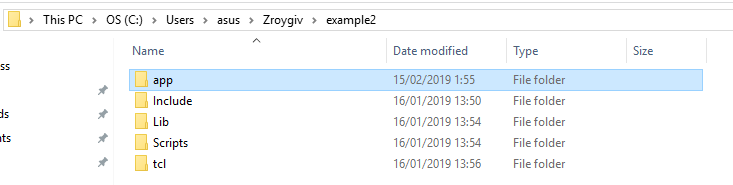
\includegraphics[width=0.85\textwidth]{figures/12/fu.PNG}}
	\caption{Folder Users}
	\label{fig:fu}
\end{figure}

\item Dalam folder app, terdapat dua folder yang bernama static dan template seperti pada gambar \ref{fig:fa}.
\begin{figure}[!htbp]
	\centerline{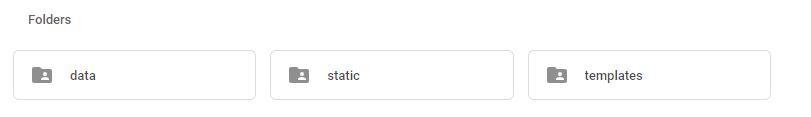
\includegraphics[width=0.85\textwidth]{figures/12/fa.PNG}}
	\caption{Folder App}
	\label{fig:fa}
\end{figure}

\item Kedua folder itu nantinya akan diisi oleh template dan juga data dari Brainwave Sinyal Web Service. 
\item Di dalam folder app, buatlah file python yang bernama flasklivechart.py, lalu isikan file tersebut dengan kode seperti pada listing \ref{lst:flc}:
\lstinputlisting[caption=Flask Live Chart,label={lst:flc}]{src/12/flc.py}
\end{enumerate}

\subsection{Sebelum membuat file JSON, buatlah folder js dan img di dalam folder static}

Seperti pada gambar \ref{fig:fs}.
\begin{figure}[!htbp]
	\centerline{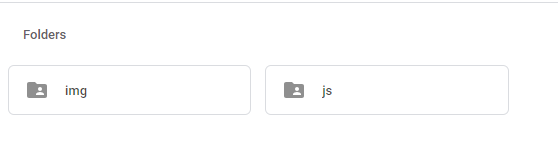
\includegraphics[width=0.85\textwidth]{figures/12/fs.PNG}}
	\caption{Folder Static}
	\label{fig:fs}
\end{figure}
\begin{enumerate}
\item Dalam folder js, buatlah file yang bernama highcharts.js, kemudian isikan kode seperti pada listing \ref{lst:hcs}:
\lstinputlisting[caption=Highcharts.js,label={lst:hcs}]{src/12/highcharts.js}

\item Dan untuk folder img, masukan gambar untuk yang nantinya akan ditampilkan pada template HTML. Adapun gambar yang dimasukkan adalah seperti pada gambar \ref{fig:eeg}.
\begin{figure}[!htbp]
	\centerline{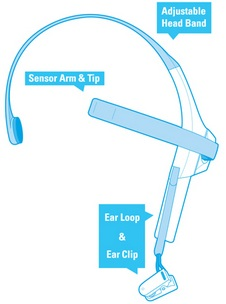
\includegraphics[width=0.85\textwidth]{figures/12/eeg.PNG}}
	\caption{EEG}
	\label{fig:eeg}
\end{figure}

\begin{figure}[!htbp]
	\centerline{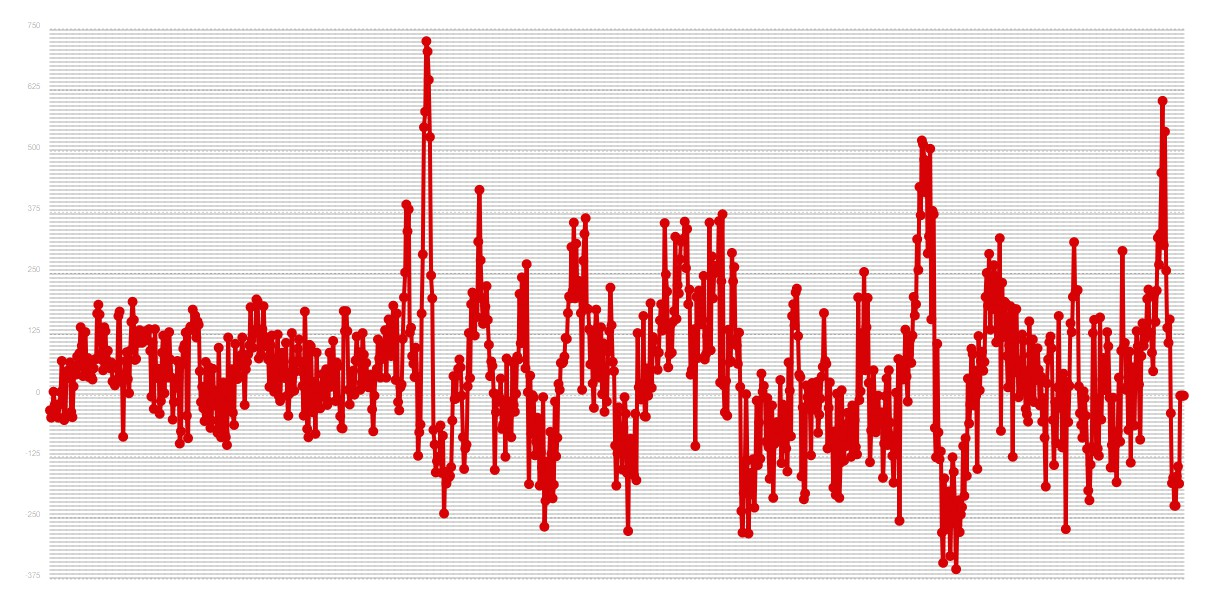
\includegraphics[width=0.85\textwidth]{figures/12/charts.PNG}}
	\caption{Charts}
	\label{fig:charts}
\end{figure}

\item Untuk menjalankan aplikasi, dibutuhkan template html untuk menjalankannya. Semua file HTML disimpan di folder templates. Terdapat empat buat file HTML yang nantinya akan dijadikan templates.
\item Template pertama, buatlah file files.html dengan kode seperti pada listing \ref{lst:flshtml}:
\lstinputlisting[caption=Files.html,label={lst:flshtml}]{src/12/files.html}
\end{enumerate}

\subsection{Dan file keempat, buatlah file HTML yang bernama live.html, kemudian isikan kode seperti pada listing \ref{lst:lvhtml}:}
\lstinputlisting[caption=live.html,label={lst:lvhtml}]{src/12/live.html}

\begin{enumerate}
\item Jika semua urusan kode sudah selesai, maka saatnya untuk menjalankan aplikasi. Untuk menjalankannya bukalah CMD, masuk ke python, kemudian masuk ke direktori tempat menyimpan semua file yang telah dibuat 
\item Masukkan perintah seperti pada listing \ref{lst:pth}:
\lstinputlisting[caption=Perintah,label={lst:pth}]{src/12/pth.py}

\item Kemudian enter.
\item Jika muncul berupa link http://localhost:5000/, salin link tersebut dan tempel di browser. Maka hasilnya akan seperti pada gambar \ref{fig:haa}.
\begin{figure}[!htbp]
	\centerline{
\includegraphics[width=0.85\textwidth]{figures/12/haa.PNG}}
	\caption{Halaman Awal Aplikasi}
	\label{fig:haa}
\end{figure}

Hasilnya seperti pada gambar \ref{fig:hd}.
\begin{figure}[!htbp]
	\centerline{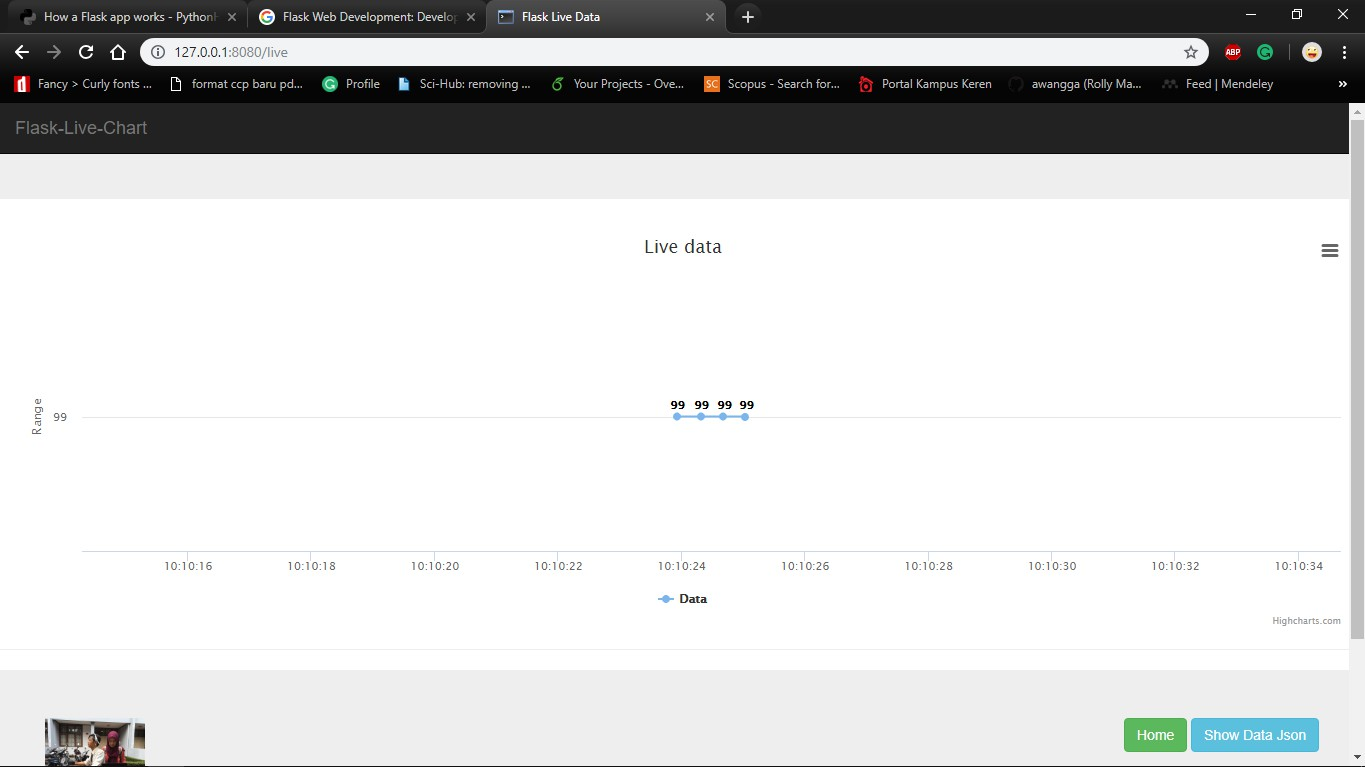
\includegraphics[width=0.85\textwidth]{figures/12/hd.PNG}}
	\caption{Hasil Data}
	\label{fig:hd}
\end{figure}

\item Pada gambar \ref{fig:haa}, data yang muncul tidak berupa gelombang dikarenakan tidak adanya inputan data yang masuk. Data akan muncul jika aplikasi dijalankan sambil memakai EEG.
\end{enumerate}